\begin{frame}{Higgs Boson Production Mechanisms}
    \begin{columns}[T] 
        \begin{column}{0.5\textwidth}
            \centering
            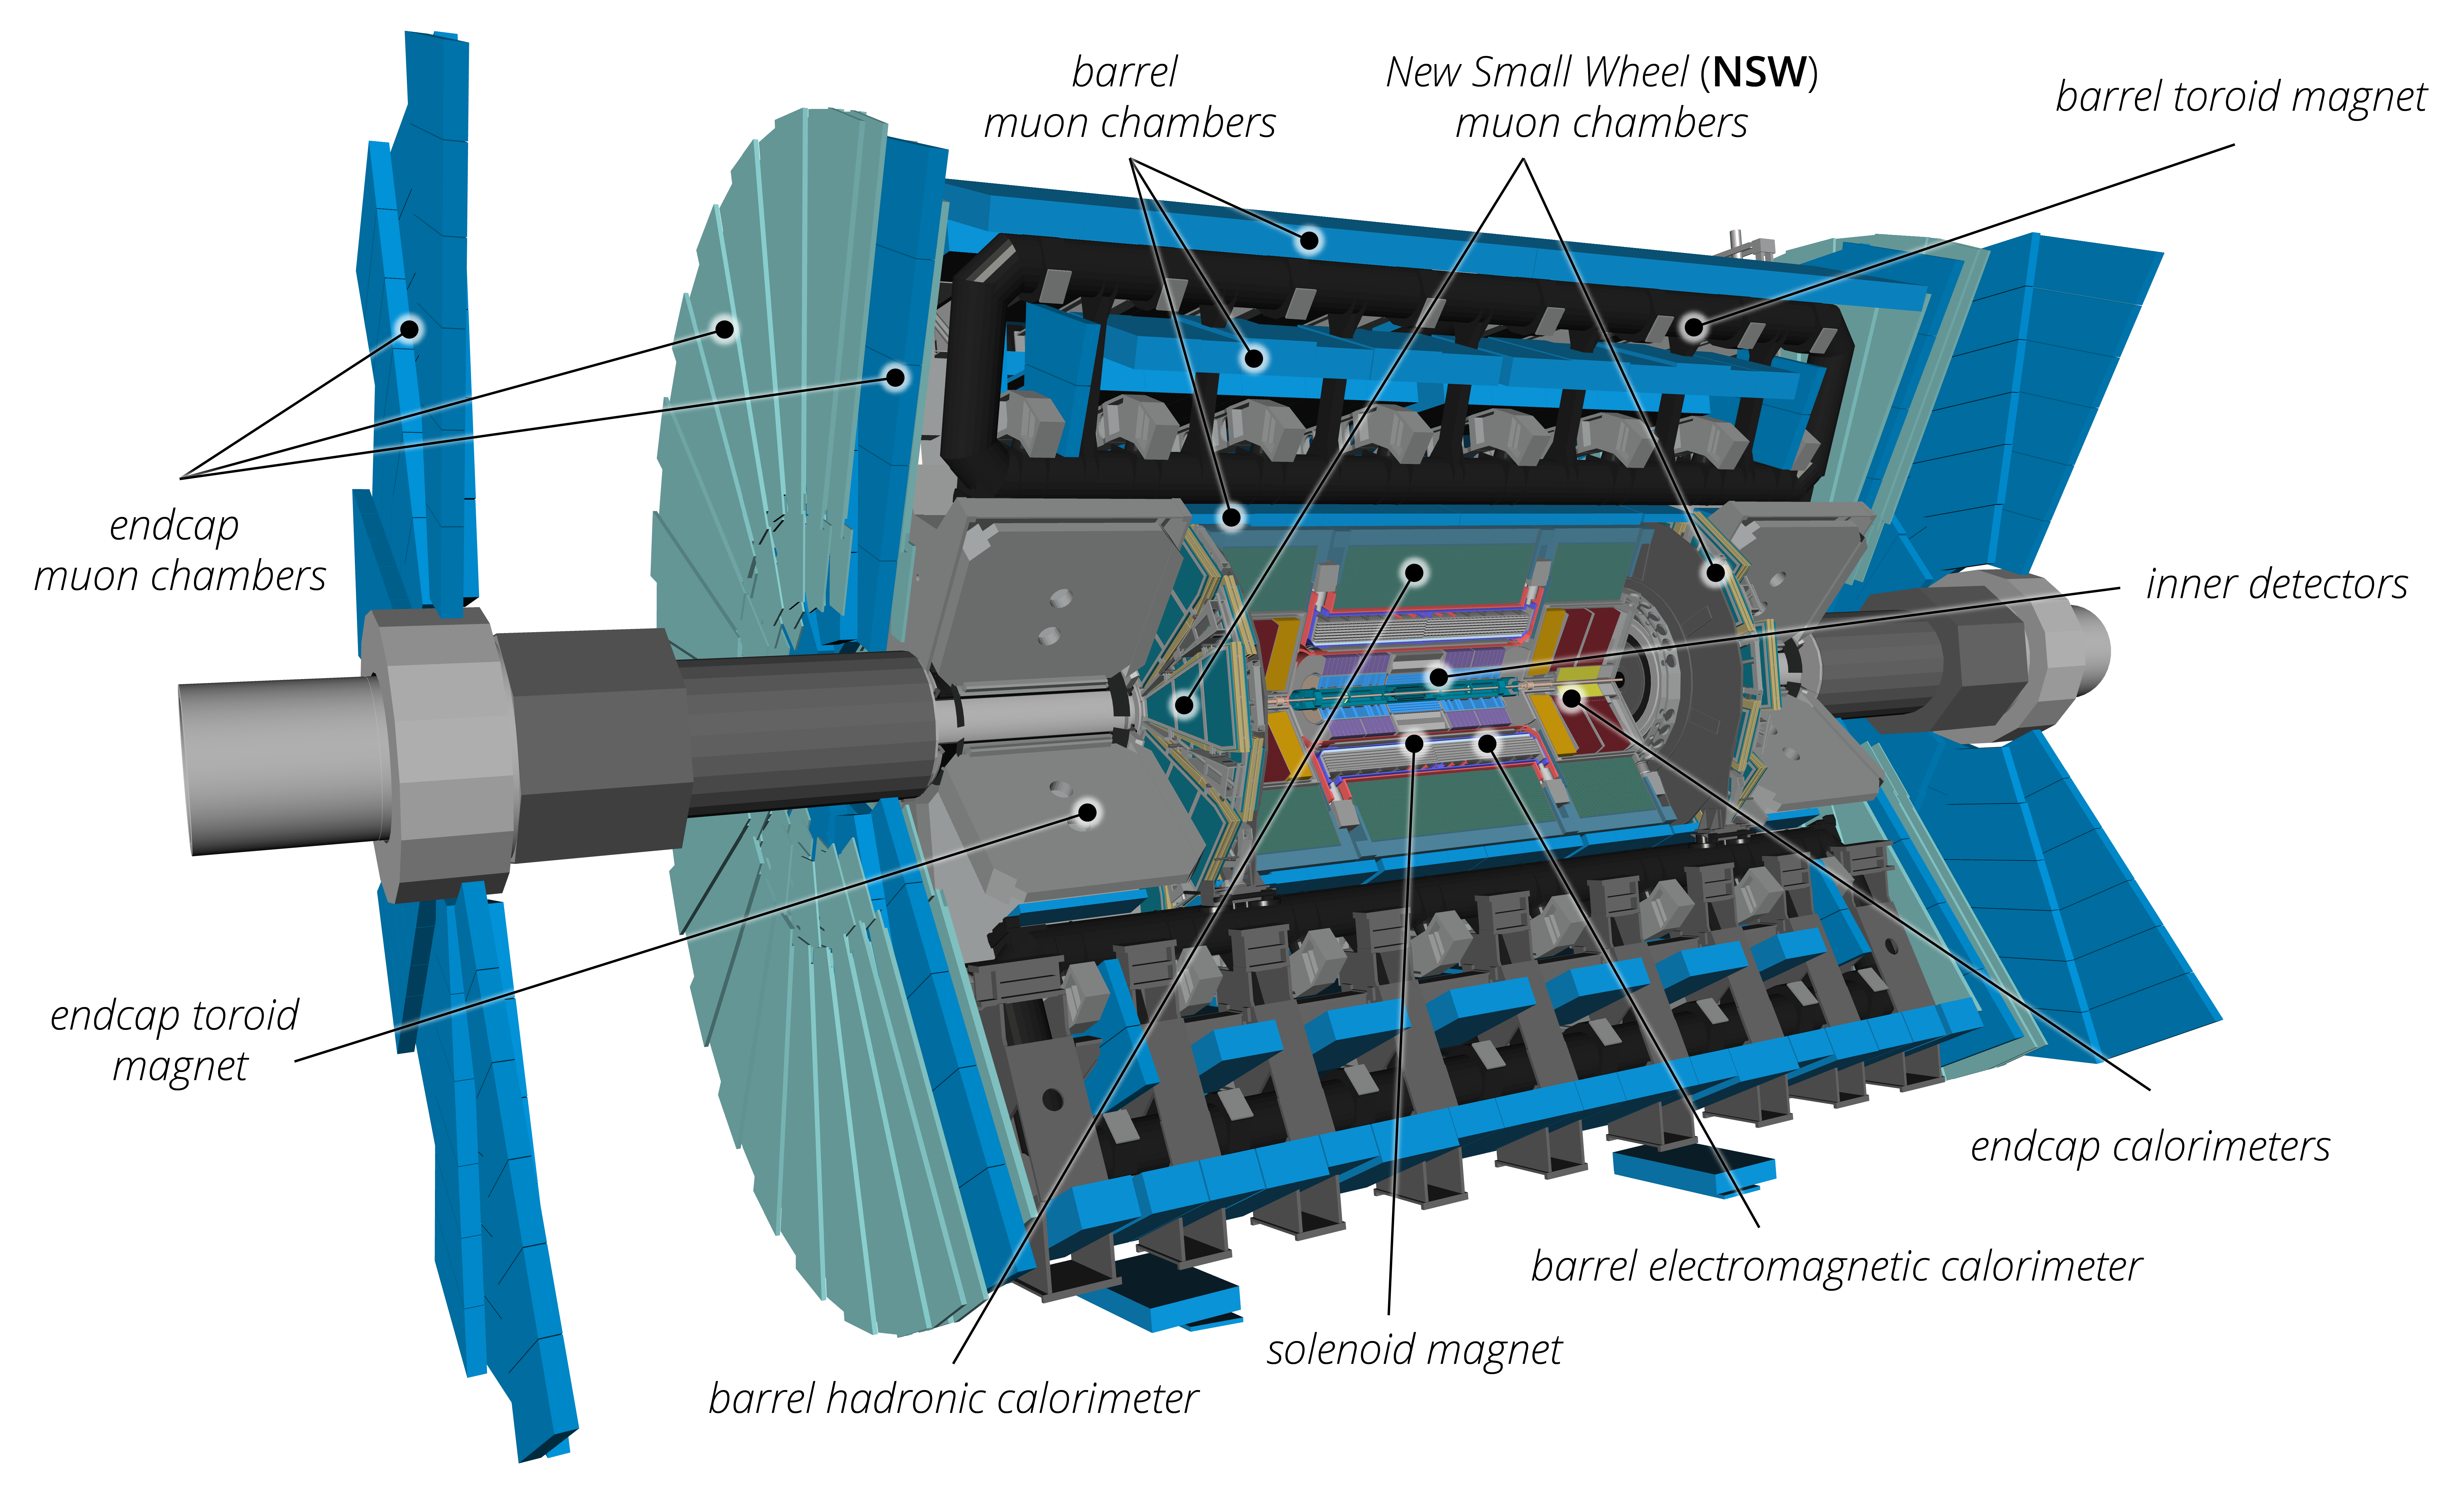
\includegraphics[width=\textwidth, keepaspectratio]{Immagini/fig_02.png}
            
            \vspace{0.47cm} 
            \tiny{\href{https://atlas.cern/Resources/Schematics}{Source: atlas.cern}}
        \end{column}
        
        \begin{column}{0.5\textwidth}
            \centering
            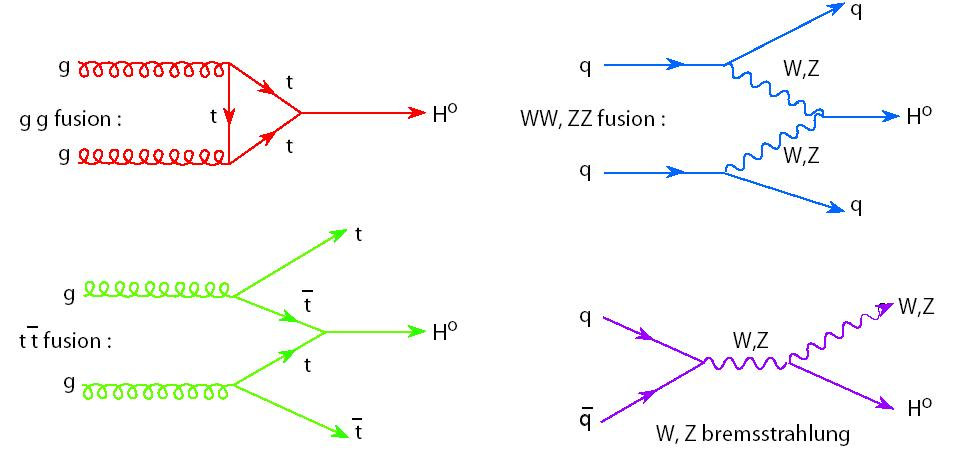
\includegraphics[width=\textwidth, keepaspectratio]{Immagini/Higgs_prod_graphs_new2.jpg}
            
            \vspace{1.4cm}
            \tiny{\href{https://sites.uci.edu/energyobserver/2012/11/26/higgs-production-and-decay-channels/}{Source: sites.uci.edu}}
        \end{column}
        
    \end{columns}
\end{frame}



% --- SLIDE 1: MC Generation Chain (Solo Testo) ---
\begin{frame}{Simulation Workflow: Monte Carlo Generation}
    \textbf{Theoretical Setup \& Generation Chain:}
    \vspace{0.3cm}
    \begin{itemize}
        \item \textbf{Hard Process:} Generation of the four main Higgs production mechanisms (ggF, VBF, WH, ZH) using \texttt{MadGraph5\_aMC@NLO}.
        \vspace{0.2cm}
        \item \textbf{Parton-Level (LHE):} Extraction of parton-level kinematics to validate the theoretical predictions and ensure consistency with known characteristics.
        \vspace{0.2cm}
        \item \textbf{Shower \& Hadronization:} Evolution of hard-scattering events via \texttt{Pythia8} to simulate parton showering, hadronization, and the production of stable particles.
        \vspace{0.2cm}
        \item \textbf{Detector Simulation:} Processing of the hadronized events through \texttt{Delphes} to accurately emulate the ATLAS detector response (efficiencies, smearing, and particle reconstruction).
    \end{itemize}
\end{frame}

% --- SLIDE 2: MC Generation Chain (Solo Grafici Parton-level) ---
\begin{frame}{Simulation Workflow: Monte Carlo Generation}
    \begin{columns}[t]
        \begin{column}{0.49\textwidth}
            \centering
            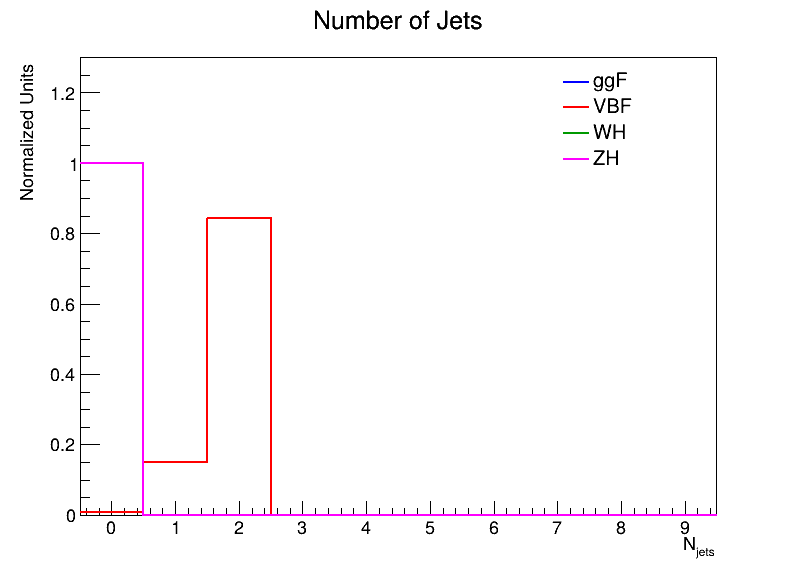
\includegraphics[width=\textwidth, keepaspectratio]{Immagini/Njets_parton_comparison.png}
        \end{column}
        \begin{column}{0.49\textwidth}
            \centering
            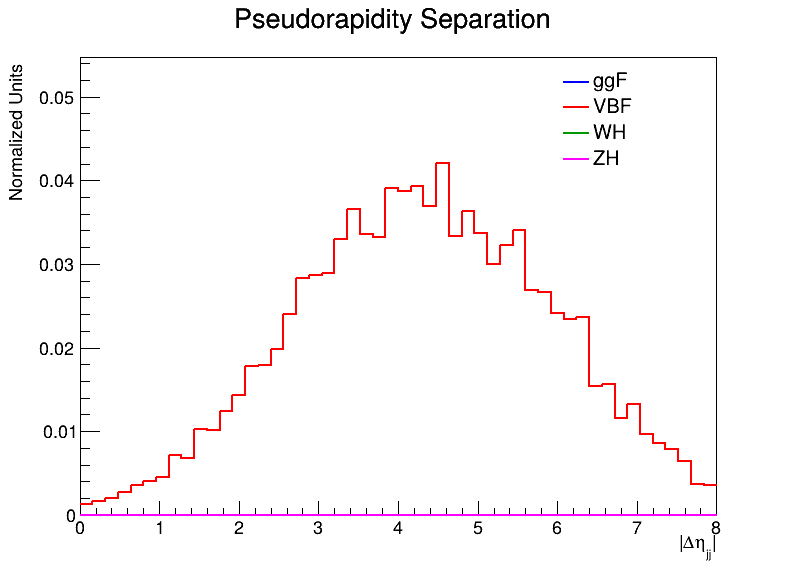
\includegraphics[width=\textwidth, keepaspectratio]{Immagini/dEta_jj_parton_comparison.png}
        \end{column}
    \end{columns}
\end{frame}

% --- SLIDE 3: Detector Level & Signatures (Solo Testo) ---
\begin{frame}{Experimental Signatures at Detector Level}
    \begin{itemize}
        \item Following the Delphes simulation, the analysis relies exclusively on reconstructed kinematic variables to mimic experimental conditions.
        \item \textbf{Signal Region (SR) Strategy:} Selection of a single, highly-discriminating variable for each mechanism to optimize the signal-to-background ratio.
        \item \textbf{Golden Variables Identified:}\\
        \vspace{0.3cm}
        \centering
            \begin{tabular}{ccc}
                \hline
                \textbf{Process} & \textbf{Key Variable} & \textbf{SR Window} \\ \hline
                \textbf{ggF} & $p_T^H$ & $[0.0, 100.0]$ GeV \\
                \textbf{VBF} & $m_{jj}$ & $[400.0, 1100.0]$ GeV \\
                \textbf{WH} & $m_T^W$ & $[0.0, 120.0]$ GeV \\
                \textbf{ZH} & $m_{ll}$ & $[80.0, 100.0]$ GeV \\ \hline
            \end{tabular}
    \end{itemize}
\end{frame}

% --- SLIDE 4: Detector Level & Signatures (ggF & VBF) ---
\begin{frame}{Experimental Signatures at Detector Level - ggF \& VBF}
    \vspace{-0.2cm}
    \begin{columns}[T] % L'opzione [T] allinea le colonne in alto
        
        % Colonna Sinistra (ggF)
        \begin{column}{0.5\textwidth}
            \centering
            \textbf{ggF Signature} \\
            \vspace{0.1cm}
            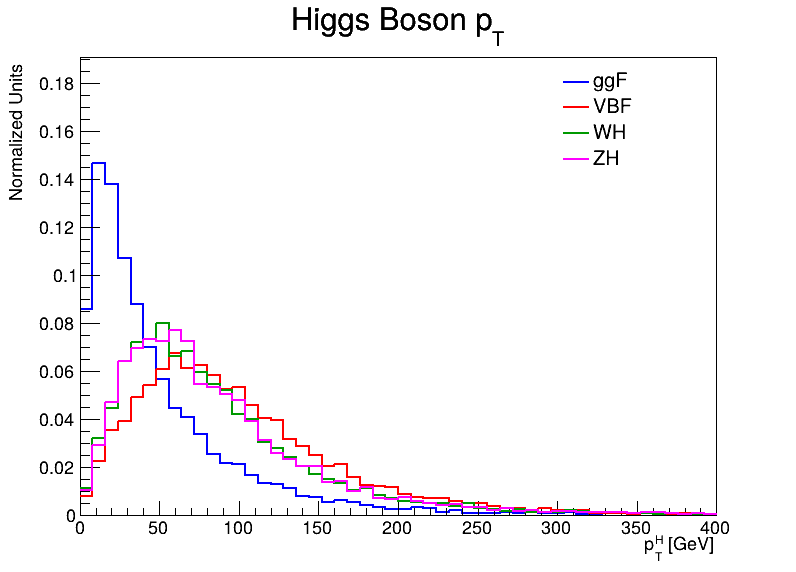
\includegraphics[width=0.95\textwidth, keepaspectratio]{Immagini/pT_H_shower_comparison.png}
        \end{column}
        
        % Colonna Destra (VBF)
        \begin{column}{0.5\textwidth}
            \centering
            \textbf{VBF Signature} \\
            \vspace{0.1cm}
            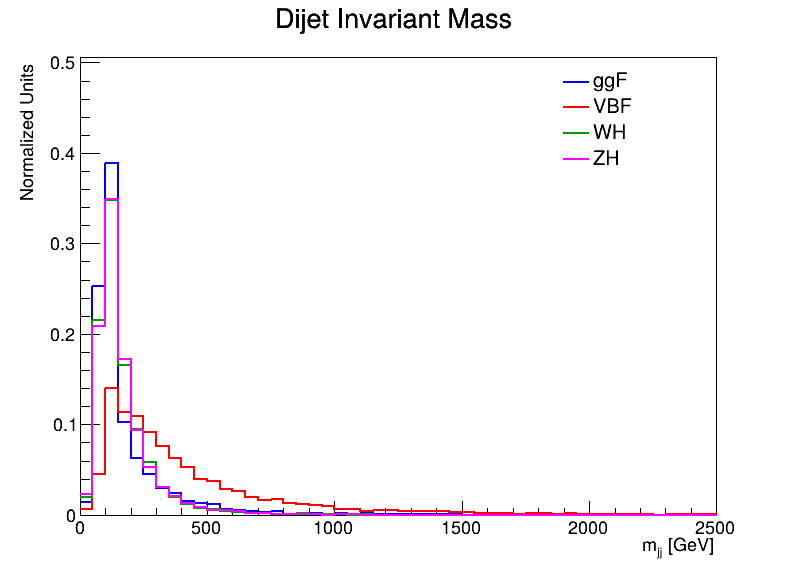
\includegraphics[width=0.95\textwidth, keepaspectratio]{Immagini/m_jj_shower_comparison.png} 
        \end{column}
        
    \end{columns}
\end{frame}

% --- SLIDE 5: Detector Level & Signatures (WH & ZH) ---
\begin{frame}{Experimental Signatures at Detector Level - WH \& ZH}
    \vspace{-0.2cm}
    \begin{columns}[T]
        
        % Colonna Sinistra (WH)
        \begin{column}{0.5\textwidth}
            \centering
            \textbf{WH Signature} \\
            \vspace{0.1cm}
            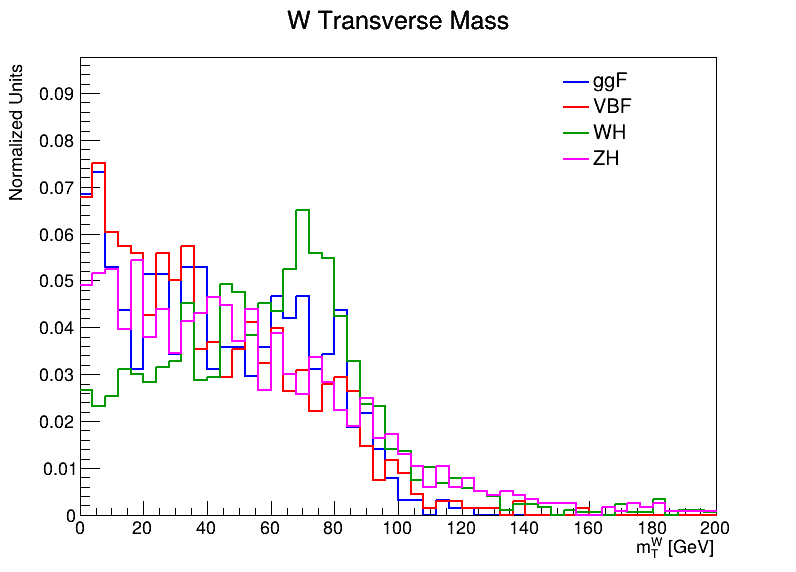
\includegraphics[width=0.95\textwidth, keepaspectratio]{Immagini/m_WT_shower_comparison.png}
        \end{column}
        
        % Colonna Destra (ZH)
        \begin{column}{0.5\textwidth}
            \centering
            \textbf{ZH Signature} \\
            \vspace{0.1cm}
            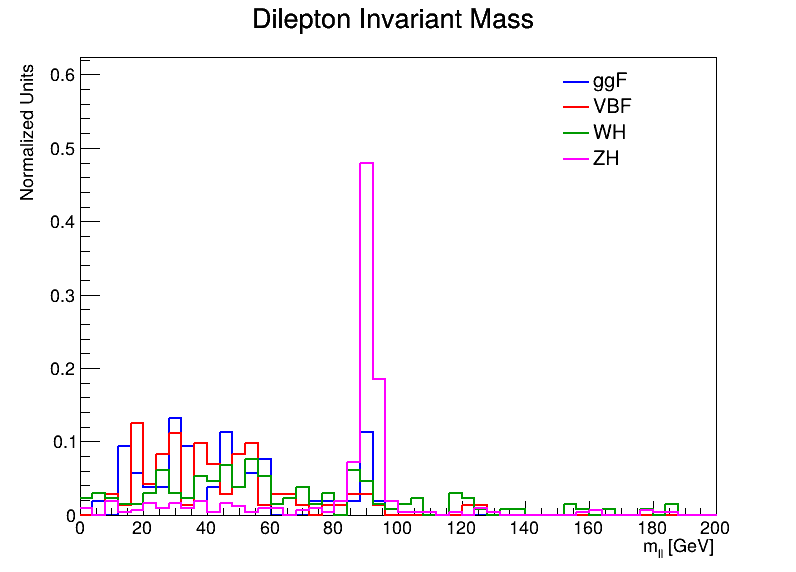
\includegraphics[width=0.95\textwidth, keepaspectratio]{Immagini/m_ll_shower_comparison.png}
        \end{column}
        
    \end{columns}
\end{frame}

\begin{frame}{Deep Dive: Vector Boson Fusion (VBF) Topology}
    \begin{columns}[T]
        
        % Colonna Sinistra: Risposte ai 3 punti chiave
        \begin{column}{0.63\textwidth}
            \small
            \textbf{Background Classification for VBF:}
            \begin{itemize}
                \item \textbf{Irreducible Background:} \textit{ggF + $\ge 2$ jets}. Same experimental final state.
                \item \textbf{Reducible Backgrounds:} \textit{WH / ZH} associated production. 
            \end{itemize}
            
            \textbf{Key Separating Observables:}
            \begin{itemize}
                \item \textbf{$\Delta\eta_{jj}$:} Large pseudorapidity gap.
                \item \textbf{$m_{jj}$:} Hard invariant mass.
            \end{itemize}
            
            \textbf{Decay-Independent Features:}
            \begin{itemize}
                \item The kinematic properties of the forward-backward tagging jets ($m_{jj}$, $\Delta\eta_{jj}$) depend strictly on the t-channel $W/Z$ exchange of the production vertex.
            \end{itemize}
        \end{column}
        
        % Colonna Destra: Il grafico di dEta_jj
        \begin{column}{0.47\textwidth}
            \begin{figure}
                \centering
                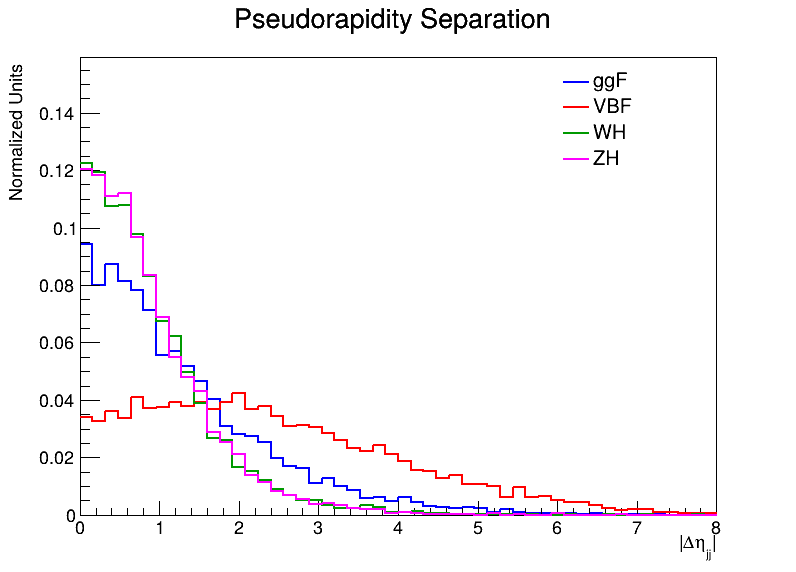
\includegraphics[width=\textwidth, keepaspectratio]{Immagini/dEta_jj_shower_comparison.png}
            \end{figure}
        \end{column}
        
    \end{columns}
\end{frame}


% --- SLIDE 7: Blind Samples Analysis (Higgs Peak) ---
\begin{frame}{Blind Samples Analysis: Higgs Reconstruction}
    \begin{columns}[T]
        \begin{column}{0.55\textwidth}
            \textbf{Analysis Strategy on Blind Samples:}
            \vspace{0.2cm}
            \begin{enumerate}
                \item \textbf{Reconstruction:} Identify the Higgs candidate via its decay products ($H \to ZZ^* \to 4\ell$).
                \vspace{0.1cm}
                \item \textbf{Mass Window:} Select events in the Higgs mass peak region ($m_{4\ell} \simeq 125$ GeV).
                \vspace{0.1cm}
                \item \textbf{Kinematics Extraction:} Build distributions for the associated objects (jets, extra leptons, $E_T^{\text{miss}}$).
                \vspace{0.1cm}
                \item \textbf{Template Matching:} Compare with MadGraph MC expectations to deduce the production mechanism.
            \end{enumerate}
        \end{column}
        
        \begin{column}{0.45\textwidth}
            \centering
            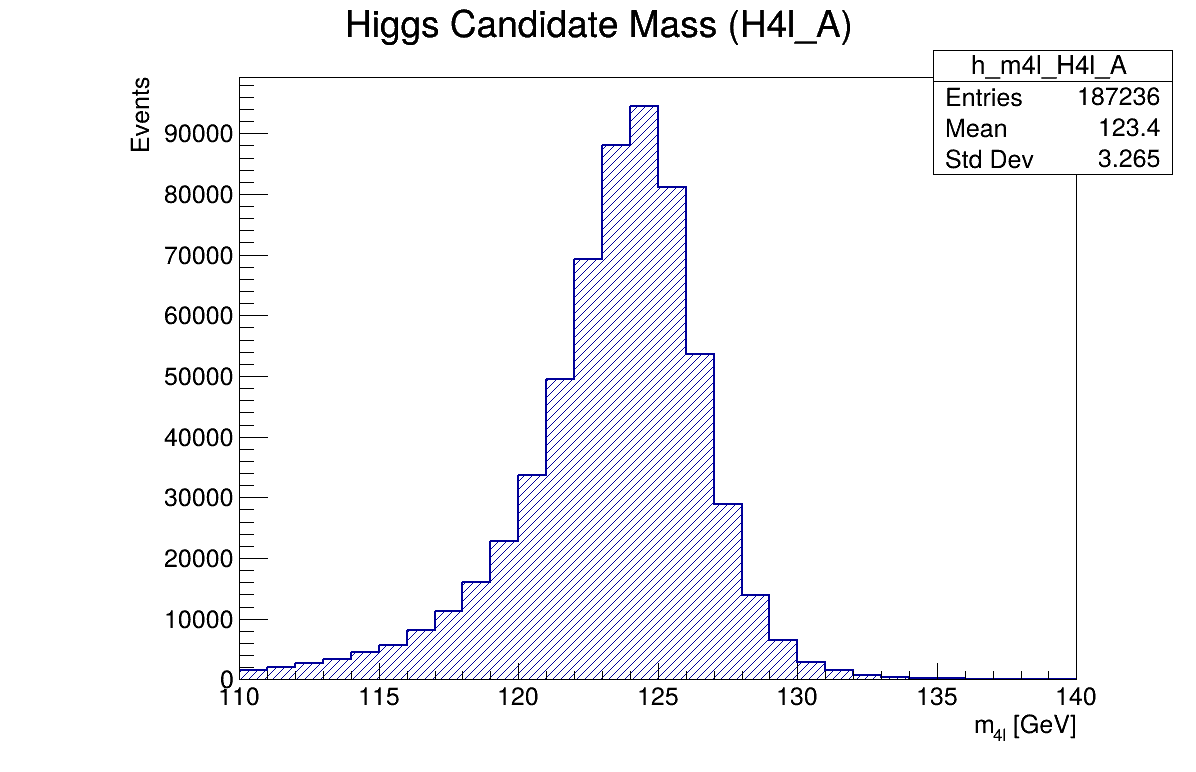
\includegraphics[width=\textwidth, keepaspectratio]{Immagini/H4l_A_m4l.png}
            
            \vspace{0.2cm}
            \footnotesize{Invariant mass $m_{4\ell}$ for Sample A clearly showing the Higgs peak.}
        \end{column}
    \end{columns}
\end{frame}

% --- SLIDE 8: Signal Regions & VBF match ---
\begin{frame}{Signal Regions \& VBF Identification}
    \begin{columns}[T]
        \begin{column}{0.45\textwidth}
            \textbf{Signal Regions Recall:}
            \begin{itemize}
                \item \textbf{VBF:} $m_{jj} \in [400, 1100]$ GeV
                \item \textbf{ggF:} $p_T^H \in [0, 100]$ GeV
                \item \textbf{ZH:} $m_{\ell\ell} \in [80, 100]$ GeV
                \item \textbf{WH:} $m_T^W \in [0, 120]$ GeV
            \end{itemize}
            
            \vspace{0.6cm}
            \textbf{Identifying VBF (Sample A):} \\
            \vspace{0.2cm}
            The dijet invariant mass ($m_{jj}$) shows excellent shape agreement with the VBF MC template in the high-mass signal region, successfully isolating the signature from irreducible backgrounds.
        \end{column}
        
        \begin{column}{0.55\textwidth}
            \centering
            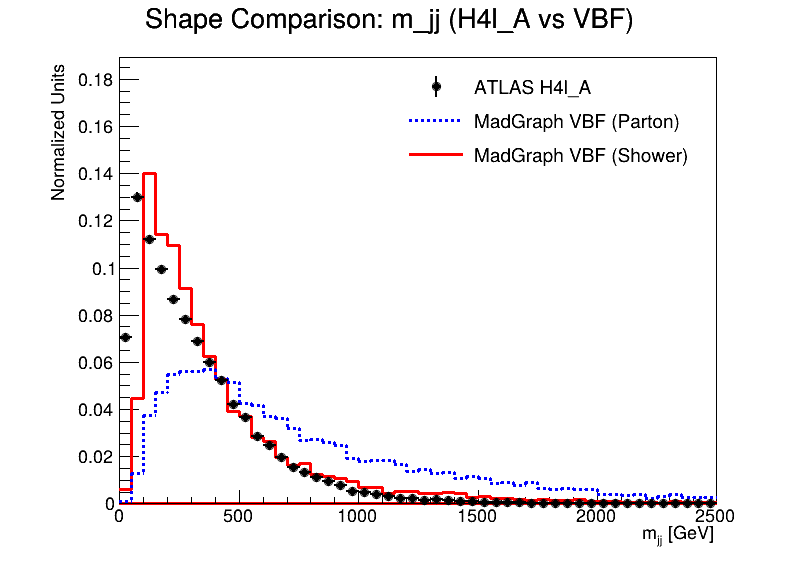
\includegraphics[width=\textwidth, keepaspectratio]{Immagini/compare_m_jj_H4l_A_vs_VBF.png}
        \end{column}
    \end{columns}
\end{frame}

% --- SLIDE 9: Identifying ggF, ZH, WH ---
\begin{frame}{Kinematic Matching for ggF, ZH, and WH}
    \vspace{-0.2cm}
    \textbf{Identifying the remaining blind samples:}
    \vspace{0.2cm}
    \begin{columns}[T]
        \begin{column}{0.33\textwidth}
            \centering
            \textbf{ggF (Sample B)} \\
            \vspace{0.1cm}
            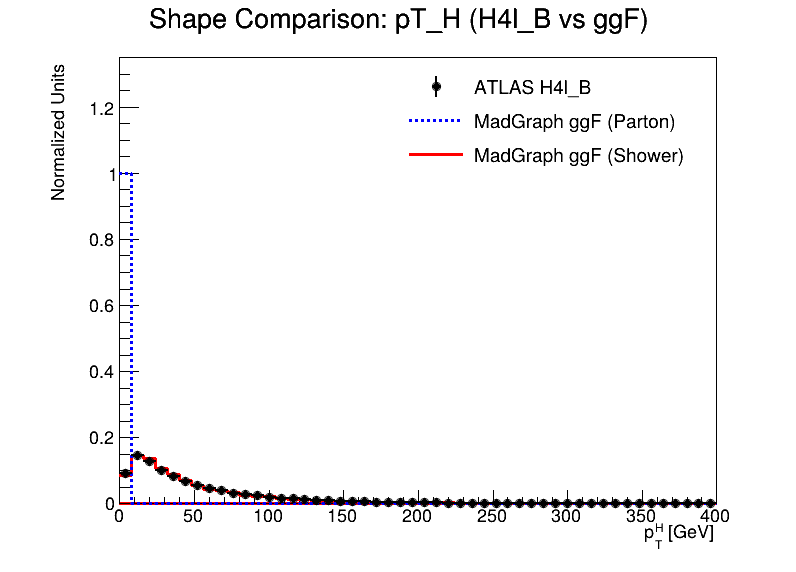
\includegraphics[width=\textwidth, keepaspectratio]{Immagini/compare_pT_H_H4l_B_vs_ggF.png} \\
            \footnotesize{Key Variable: $p_T^H$}
        \end{column}
        
        \begin{column}{0.33\textwidth}
            \centering
            \textbf{ZH (Sample C)} \\
            \vspace{0.1cm}
            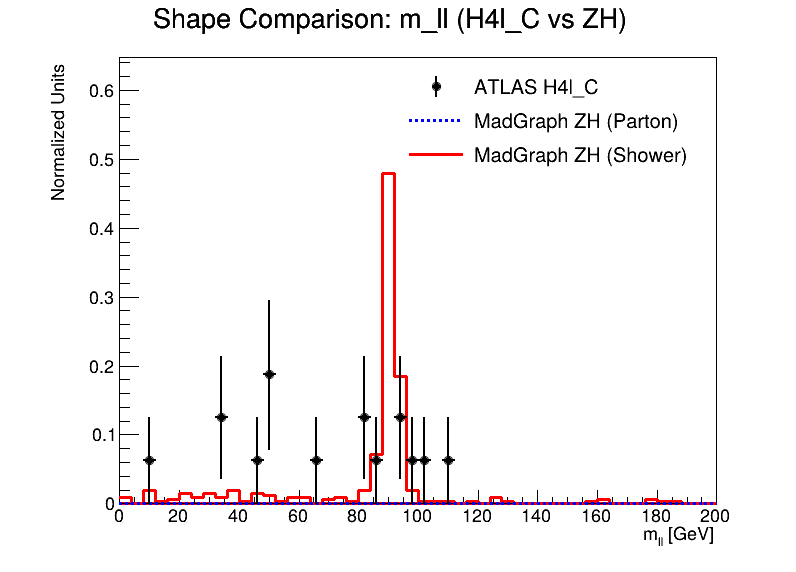
\includegraphics[width=\textwidth, keepaspectratio]{Immagini/compare_m_ll_H4l_C_vs_ZH.png} \\
            \footnotesize{Key Variable: $m_{\ell\ell}$}
        \end{column}
        
        \begin{column}{0.33\textwidth}
            \centering
            \textbf{WH (Sample D)} \\
            \vspace{0.1cm}
            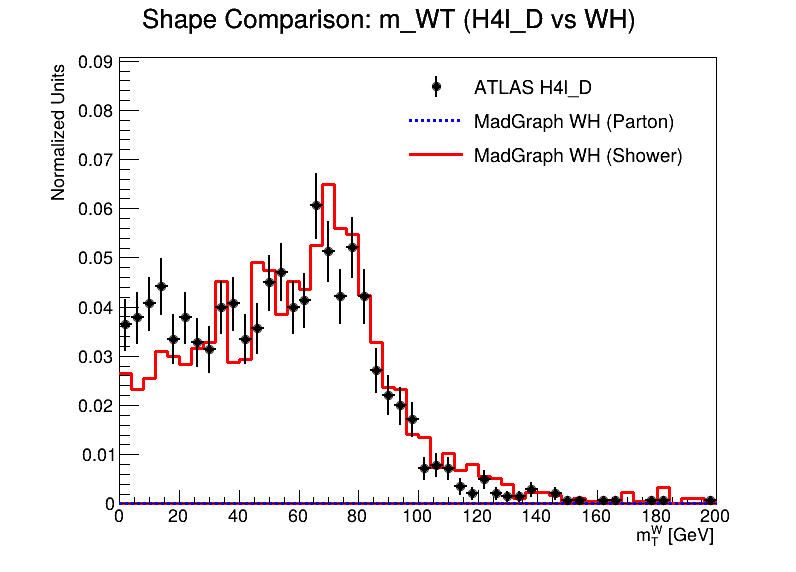
\includegraphics[width=\textwidth, keepaspectratio]{Immagini/compare_m_WT_H4l_D_vs_WH.png} \\
            \footnotesize{Key Variable: $m_T^W$}
        \end{column}
    \end{columns}
    
    \vspace{0.4cm}
    \centering
    \small{Each sample exhibits strong shape compatibility with its respective MC expectation within the specifically defined Signal Region.}
\end{frame}

% --- SLIDE 10: Statistical Validation ---
\begin{frame}{Statistical Validation ($\chi^2$ Shape Test)}
    To quantitatively confirm the visual matches, a $\chi^2$ shape test was performed comparing the Data samples to the MC templates in the corresponding Signal Regions.
    
    \vspace{0.4cm}
    \centering
    \renewcommand{\arraystretch}{1.3}
    \begin{tabular}{l c c l}
        \hline
        \textbf{Blind Sample} & \textbf{Best MC Match} & \textbf{Key Variable} & \textbf{Shape Test ($\chi^2$/NDF)} \\ \hline
        \textbf{Sample A} & VBF & $m_{jj}$ & $\mathbf{7.08}$ (Strong Match) \\
        \textbf{Sample B} & ggF & $p_T^H$ & Consistent Shape \\
        \textbf{Sample C} & ZH & $m_{\ell\ell}$ & Consistent Shape \\ 
        \textbf{Sample D} & WH & $m_T^W$ & $\mathbf{2.19}$ (Strong Match) \\ \hline
    \end{tabular}
    
    \vspace{0.6cm}
    \begin{itemize}
        \item The shape tests strongly reject the null hypotheses for mismatched combinations (e.g., Sample D vs ZH yields $\chi^2/\text{NDF} \approx 1000$).
        \item \textbf{Conclusion:} The designed kinematic discriminants successfully and reliably decouple the Higgs production mechanisms at the detector level.
    \end{itemize}
\end{frame}